\chapter{SISTEMI LINEARI E NON LINEARI}
\section{Esercizio 8}
\textit{\textbf{Descrizione:} Scrivere una function Matlab che, data in ingresso una matrice \textbf{A}, restituisca una matrice, \textbf{LU}, che contenga l'informazione sui suoi fattori \textbf{L} ed \textbf{U}, ed un vettore \textbf{p} contenente la relativa permutazione, della fattorizzazione LU con pivoting parziale di A: \textbf{function [LU,p] = palu(A)}. Curare particolarmente la scrittura e l'efficienza della function.}\newline

\emph{Soluzione:}\\~\\

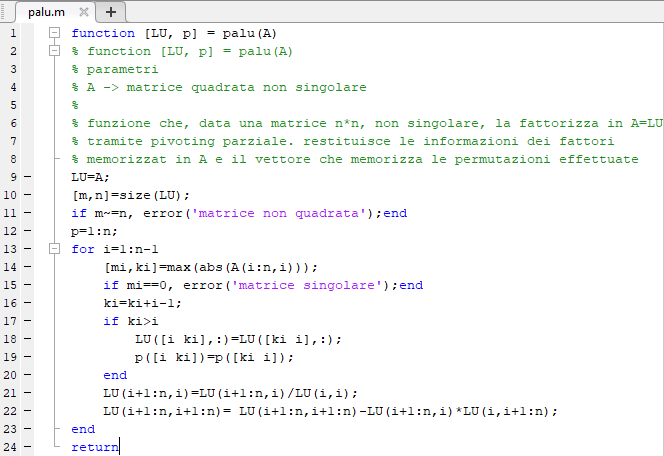
\includegraphics[width=1.3\linewidth]{img/palu}\newpage